%!TEX root = ../../paper.tex

\begin{figure*}
	\centering
	%!TEX root = ../../paper.tex

% Ferdosi 1 - MBE
\begin{subfigure}{0.3\textwidth}
	\centering
	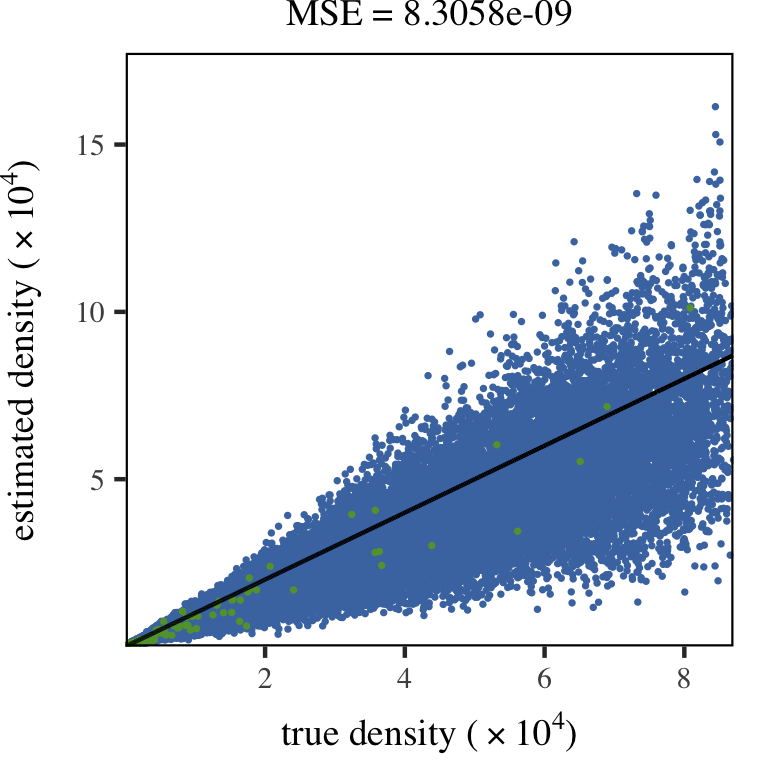
\includegraphics[keepaspectratio=true, width=\textwidth, height=0.23\textheight]{result/img/results_ferdosi_1_60000_mbe_silverman}
	\caption{Set \ferdosiOne, \mbe}
	\label{fig:results:singlesphere:mbe:ferdosi1}
\end{subfigure}
% Ferdosi 1 - SAMBE
\begin{subfigure}{0.3\textwidth}
	\centering
	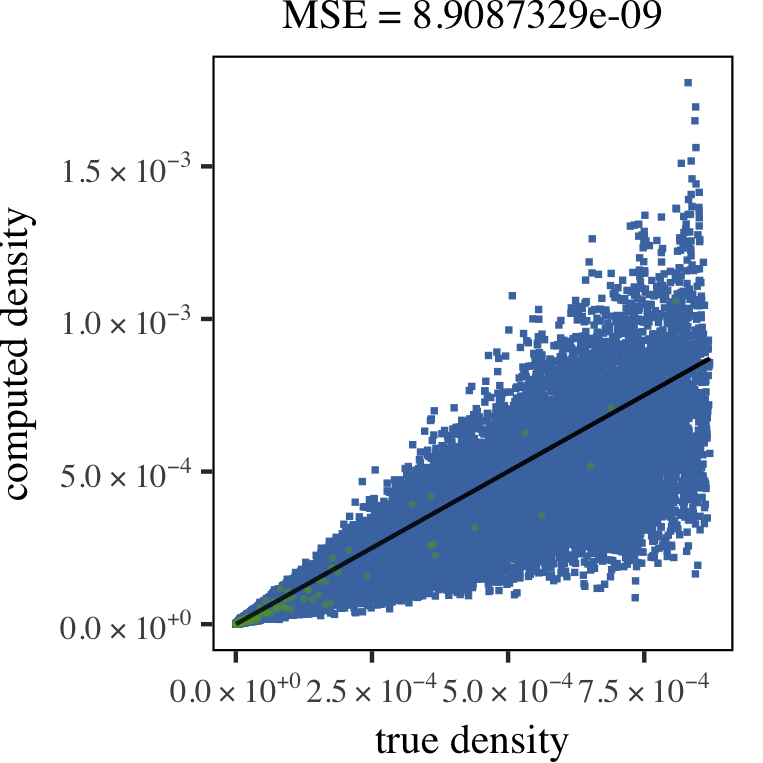
\includegraphics[keepaspectratio=true, width=\textwidth, height=0.23\textheight]{result/img/results_ferdosi_1_60000_sambe_silverman}
	\caption{Set \ferdosiOne, \sambe}
	\label{fig:results:singlesphere:sambe:ferdosi1}
\end{subfigure}
\subfigvspace
% Baakman 1	- MBE
\begin{subfigure}{0.3\textwidth}
	\centering
	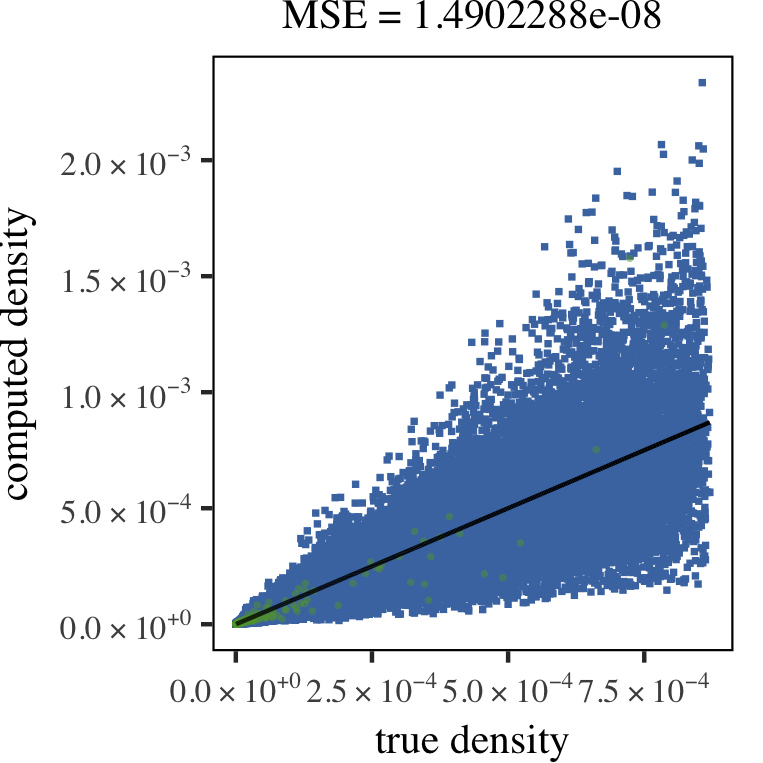
\includegraphics[keepaspectratio=true, width=\textwidth, height=0.23\textheight]{result/img/results_baakman_1_60000_mbe_silverman}
	\caption{Set \baakmanOne, \mbe}
	\label{fig:results:singlesphere:mbe:baakman1}
\end{subfigure}
% Baakman 1	- SAMBE
\begin{subfigure}{0.3\textwidth}
	\centering
	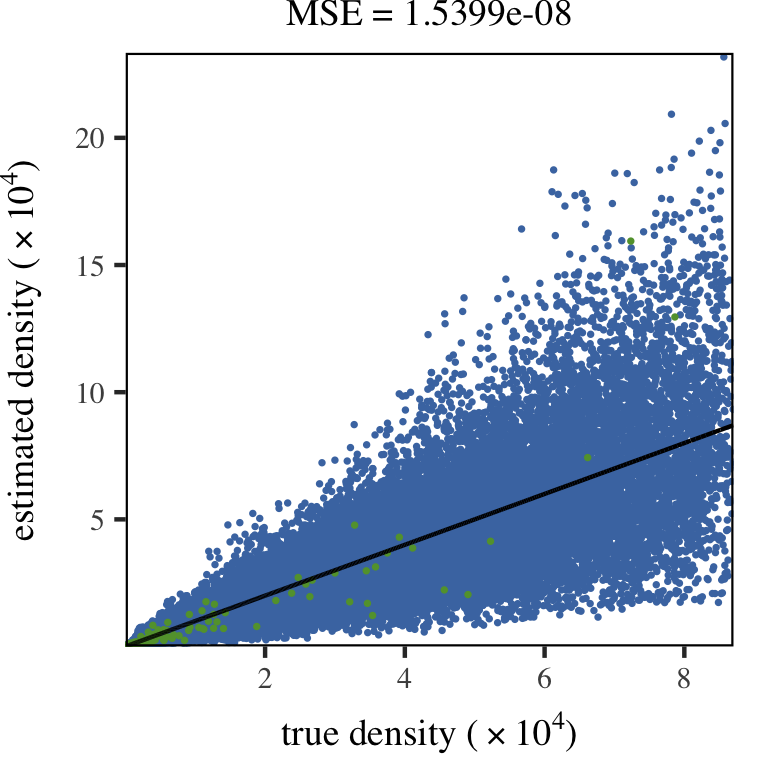
\includegraphics[keepaspectratio=true, width=\textwidth, height=0.23\textheight]{result/img/results_baakman_1_60000_sambe_silverman}
	\caption{Set \baakmanOne, \sambe}
	\label{fig:results:singlesphere:sambe:baakman1}
\end{subfigure}
\subfigvspace
% Baakman 4 - MBE
\begin{subfigure}{0.3\textwidth}
	\centering
	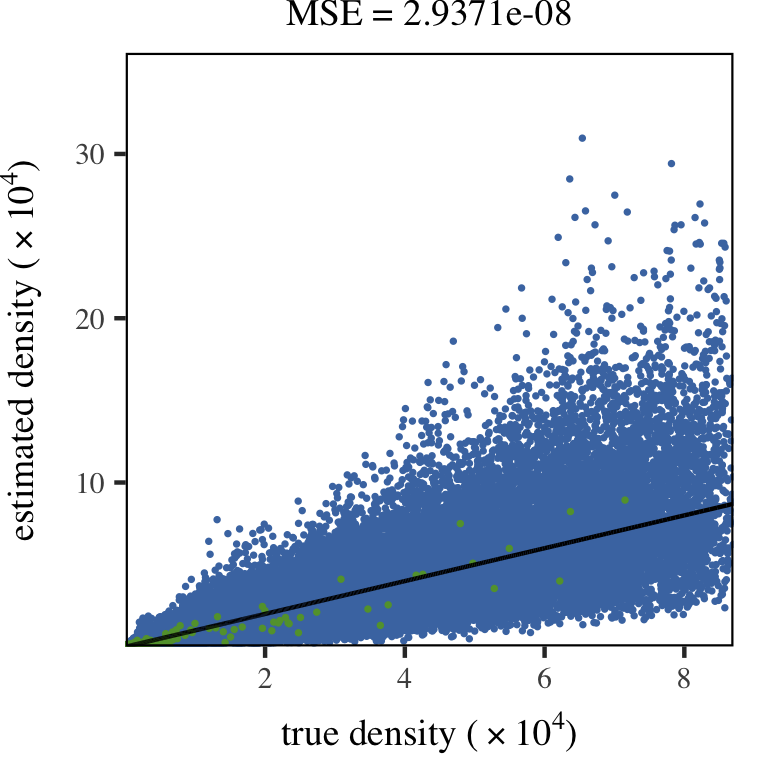
\includegraphics[keepaspectratio=true, width=\textwidth, height=0.23\textheight]{result/img/results_baakman_4_60000_mbe_silverman}
	\caption{Set \baakmanFour, \mbe}
	\label{fig:results:singlesphere:mbe:baakman4}
\end{subfigure}	
% Baakman 4 - SAMBE
\begin{subfigure}{0.3\textwidth}
	\centering
	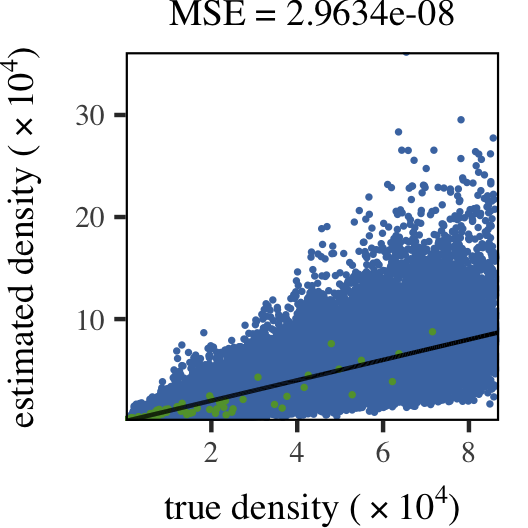
\includegraphics[keepaspectratio=true, width=\textwidth, height=0.23\textheight]{result/img/results_baakman_4_60000_sambe_silverman}
	\caption{Set \baakmanFour, \sambe}
	\label{fig:results:singlesphere:sambe:baakman4}
\end{subfigure}		
\subfigvspace
% Baakman 5 - MBE
\begin{subfigure}{0.3\textwidth}
	\centering
	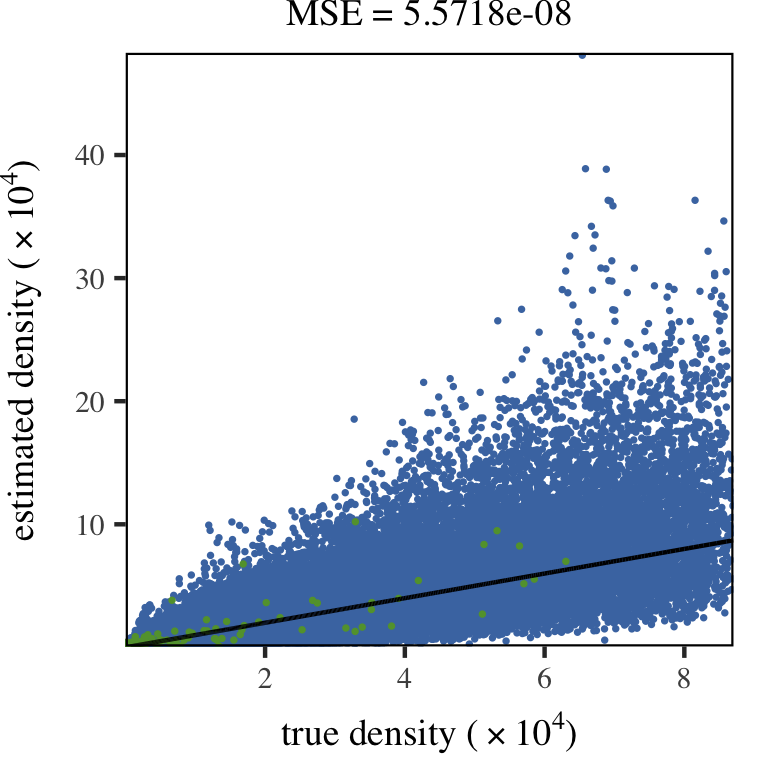
\includegraphics[keepaspectratio=true, width=\textwidth, height=0.23\textheight]{result/img/results_baakman_5_60000_mbe_silverman}
	\caption{Set \baakmanFive, \mbe}
	\label{fig:results:singlesphere:mbe:baakman5}
\end{subfigure}
% Baakman 5 - SAMBE
\begin{subfigure}{0.3\textwidth}
	\centering
	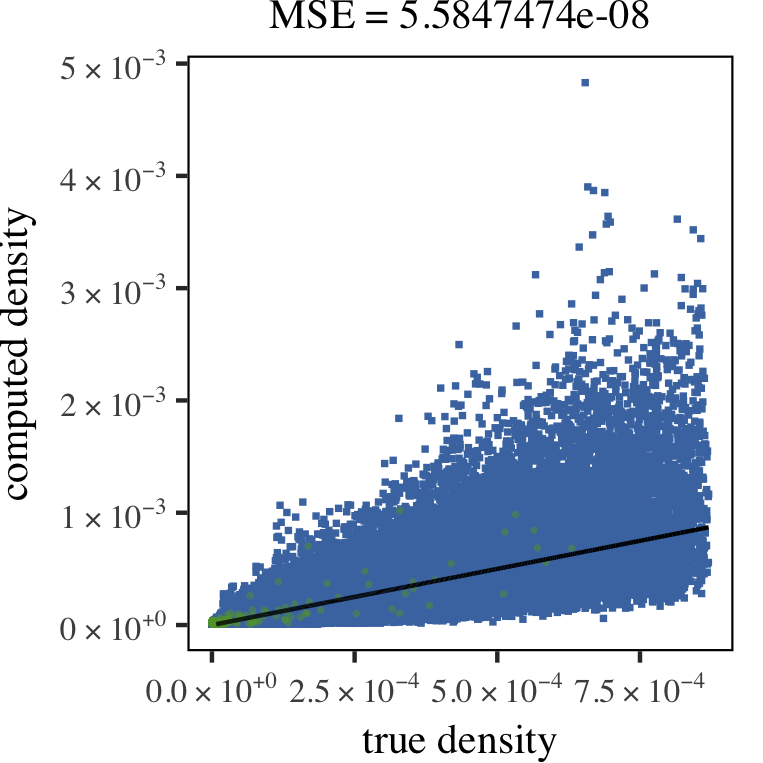
\includegraphics[keepaspectratio=true, width=\textwidth, height=0.23\textheight]{result/img/results_baakman_5_60000_sambe_silverman}
	\caption{Set \baakmanFive, \sambe}
	\label{fig:results:singlesphere:sambe:baakman5}
\end{subfigure}	
	\caption{Plot of the density as estimated by \subref{fig:results:singlesphere:mbe:ferdosi1}-\subref{fig:results:singlesphere:mbe:baakman5} \mbe and \subref{fig:results:singlesphere:sambe:ferdosi1}-\subref{fig:results:singlesphere:sambe:baakman5} \sambe as a function of the known density of the datasets with a single Gaussian.}
	\label{fig:results:singleSphere:comparativePlots}
\end{figure*}

\begin{table}
	\centering
	%!TEX root = ../../paper.tex

\begin{tabular}{l*{2}{S[scientific-notation=true, round-mode=places,round-precision=3]}}
\toprule
~ 				& \multicolumn{2}{c}{Estimator}\\ \cmidrule{2-3}
Set				& {\mbe}					& {\sambe}	\\
\midrule
\ferdosiOne		& 8.30580618349064E-09		&  8.9087329457441E-09 \\
\baakmanOne		& 1.49022877061299E-08		&  1.5398737157543E-08 \\	
\baakmanFour	& 2.93709420107411E-08		&  2.9634323205557E-08 \\	
\baakmanFive	& 5.57179476550916E-08		&  5.5847473903432E-08 \\	
\bottomrule
\end{tabular}
	\caption{Performance of the Modified Breiman Estimator with fixed-shaped and shape-adaptive kernels on the datasets with a single Gaussian.} 	
	\label{tab:results:singleSphere:mse}
\end{table}

\begin{table}
	\centering
	%!TEX root = ../../paper.tex

% \sisetup{
% 	table-format=1.3e+1,
% 	scientific-notation=true, 
% 	table-number-alignment=center,
% }

% Mean and SD in single column
% \begin{tabular}{@{}c*{6}{c}@{}}
% \toprule
% ~				& Full Set 												& \legendComponentOne Gaussian 1						& \legendComponentTwo Gaussian 2						& \legendComponentThree Gaussian 3						& \legendComponentFour Gaussian 4					 	&  \legendComponentNoise Noise\\
% \midrule
% %
% \ferdosiTwo		& \meanSD{1.504005042371507e+00}{5.309582791641542e-01} & \meanSD{1.320121582169093e+00}{1.749869852989719e-01} & \meanSD{1.304784013773833e+00}{1.427734068384871e-01} & ~ 													& ~ 													& \meanSD{1.890276960903559e+00}{7.587403345342156e-01}\\
% \baakmanTwo 	& \meanSD{1.614716145373154e+00}{5.702499690627806e-01} & \meanSD{1.407377455694081e+00}{2.782480127488867e-01} & \meanSD{1.491043432778090e+00}{3.453168397321122e-01}	& ~ 													& ~ 													& \meanSD{11.948464282370670e+00}{7.826307984091438e-01}\\
% \ferdosiThree	& \meanSD{1.460357930082488e+00}{5.507084955708148e-01} & \meanSD{1.294023549845817e+00}{1.889517285607608e-01} & \meanSD{1.265946347671562e+00}{1.301150512342848e-01} & \meanSD{1.291829938425150e+00}{2.103396722315814e-01} & \meanSD{1.275739356043035e+00}{1.654855348814119e-01} & \meanSD{1.819950324176552e+00}{8.111641695146756e-01} \\
% \baakmanThree 	& \meanSD{1.532493079967588e+00}{5.713672219810757e-01} & \meanSD{1.314980484677339e+00}{2.190657831683435e-01} & \meanSD{1.487242917765238e+00}{3.393090417977690e-01} & \meanSD{1.291829938425150e+00}{2.103396722315814e-01} & \meanSD{1.396015162355687e+00}{2.851380764085146e-01} & \meanSD{1.854880861700560e+00}{8.195085323228068e-01}\\
% %
% \bottomrule
% \end{tabular}

\small
\sisetup{
	table-format=1.4,
	scientific-notation=fixed,
	table-number-alignment=center,
	fixed-exponent=0,
	round-mode=figures,
	round-precision=4
}


\begin{tabular}{@{}c*{12}{S}@{}}
\toprule
 				& \multicolumn{2}{c}{~} 						& \multicolumn{2}{c}{\legendComponentOne Gaussian 1} 	& \multicolumn{2}{c}{\legendComponentTwo Gaussian 2}	& \multicolumn{2}{c}{\legendComponentThree Gaussian 3}	& \multicolumn{2}{c}{\legendComponentFour Gaussian 4}	& \multicolumn{2}{c}{\legendComponentNoise Noise} \\
															  	\cmidrule(lr){4-5}							  				\cmidrule(lr){6-7}							  			\cmidrule(lr){8-9} 							  			\cmidrule(lr){10-11} 							  \cmidrule(lr){12-13}
~				& {\mean}				& {\SD}			& {\mean}				 & {\SD}			& {\mean}				 & {\SD}			 & {\mean}				& {\SD}			& {\mean}				& {\SD}			& {\mean}					& {\SD}\\ 			
\midrule
\ferdosiTwo		& 1.504005042371507e+00 & 5.309582791641542e-01 & 1.320121582169093e+00 & 1.749869852989719e-01 & 1.304784013773833e+00 & 1.427734068384871e-01 &  						&  						& 	 					&  							& 1.890276960903559e+00 	& 7.587403345342156e-01\\
\baakmanTwo 	& 1.614716145373154e+00 & 5.702499690627806e-01 & 1.407377455694081e+00 & 2.782480127488867e-01 & 1.491043432778090e+00 & 3.453168397321122e-01 &  						&  						& 	 					&  							& 1.948464282370670e+00 	& 7.826307984091438e-01\\
\ferdosiThree 	& 1.460357930082488e+00 & 5.507084955708148e-01 & 1.294023549845817e+00 & 1.889517285607608e-01 & 1.265946347671562e+00 & 1.301150512342848e-01 & 1.291829938425150e+00 & 2.103396722315814e-01 & 1.275739356043035e+00 & 1.654855348814119e-01 	& 1.819950324176552e+00 	& 8.111641695146756e-01 \\
\baakmanThree 	& 1.532493079967588e+00 & 5.713672219810757e-01 & 1.314980484677339e+00 & 2.190657831683435e-01 & 1.487242917765238e+00 & 3.393090417977690e-01 & 1.291829938425150e+00 & 2.103396722315814e-01 & 1.396015162355687e+00 & 2.851380764085146e-01 	& 1.854880861700560e+00 	& 8.195085323228068e-01\\
\bottomrule
\end{tabular}
	\caption{The mean and the standard deviation of the anisotropy of the kernels used for the dataset with a single Gaussian.}
	\label{tab:results:singleSphere:anisotropy}
\end{table}

This section compares the performance of the Modified Breiman Estimator with symmetric and shape-adaptive kernels on datasets that contain one Gaussian. Comparing the mean squared errors of the \mbe with those of \sambe in \cref{tab:results:singleSphere:mse} we find that the two estimators perform comparably, but that the fixed-shape estimator always gives a slightly lower mean squared error. This is confirmed by the visualization of the results in \cref{fig:results:singleSphere:comparativePlots} where hardly any difference is visible between \cref{fig:results:singlesphere:mbe:ferdosi1,fig:results:singlesphere:mbe:baakman1,fig:results:singlesphere:mbe:baakman4,fig:results:singlesphere:mbe:baakman5}, and \cref{fig:results:singlesphere:sambe:ferdosi1,fig:results:singlesphere:sambe:baakman1,fig:results:singlesphere:sambe:baakman4,fig:results:singlesphere:sambe:baakman5}, respectively.

	% Ferdosi 1
		Comparing \cref{fig:results:singlesphere:mbe:ferdosi1} with \cref{fig:results:singlesphere:sambe:ferdosi1} we find hardly any difference between the results of the two estimators, \sambe overshoots some densities more than \mbe, but otherwise the results seem identical, which fits with the small difference in mean square error. 
		% Difference between components ?
		Reviewing the mean squared errors of the components of this dataset we find that \mbe slightly outperforms \sambe on both components.

	% Baakman 1
		\Cref{fig:results:singlesphere:mbe:baakman1,fig:results:singlesphere:sambe:baakman1} confirm the conclusion drawn from the \MSE, there is hardly any difference in performance between the two estimators. 
		% Difference between components ?
		Nor is there any difference between them within components.

	% Baakman 4
		Based on the differences between \cref{fig:results:singlesphere:mbe:baakman4,fig:results:singlesphere:sambe:baakman4} we can at best conclude that the shape-adaptive estimator overestimates the densities slightly more than the fixed-shape estimator. 
		% Difference between noise and gaussian?
		The differences between estimators within components are not significant.

	% Baakman 5
		\Cref{fig:results:singlesphere:mbe:baakman5,fig:results:singlesphere:sambe:baakman5} supports the \MSE in that hardly any difference in estimated densities between the two estimators on dataset \baakmanFive exists. 
		% Difference between noise and gaussian?
		Furthermore within components the differences between the estimators are also negligible. 

	% Algehele observatie voor single sphere datsets
		% Length of the minor axis
		We have found no direct correlation between the length of largest minor axis of the eigenellipse and the performance of the estimators, \eg the \MSE of \baakmanFour is lower than that of \baakmanOne. 
		% Length of the major axis
		Comparing the performance of both estimators on between dataset \ferdosiOne and \baakmanFive suggest that lengthening the major axes has a negative influence on the performance of the estimator. 
